\section{Joint seed choices and exact scale reuse}
\label{sec:joint-policy}
The preceding study reduces unnecessary equation generation, but some sparse choices still require a repeated calculation. To reduce this cost, we train new policies that select a seed boundary and Kira configuration together, then compare them with the preceding ML application. Validation retains the preceding application for both graphs because neither replacement clears the required improvement threshold. We add an exact scaling relation that reuses a completed reduction at a different overall momentum scale. The retained ML application performs the first reduction, and the exact identity can remove later reductions with matching dimensionless kinematics.

\subsection{Learning a complete reduction configuration}
The candidate configurations combine sparse boundaries with Kira's integral-ordering and internal propagator-permutation options~\cite{Kira2,Kira3}. The model chooses a configuration before equation generation. Kira then uses its native elimination procedure, and the earlier learned row policy remains omitted. Development reductions determine the candidate set, while separate training reductions supply the complete time of each candidate, including failed attempts and recovery. This follows the same cost-based principle as the preceding seed-boundary study; sparse seed searches also motivate the work in Ref.~\cite{TubeSeeding2026}.

We compare regression trees, random forests, and extremely randomized trees~\cite{CART1984,Breiman2001Forest,Geurts2006ExtraTrees}. Each predicts candidate log-time ratios from 68 features describing the integral family and target powers. Validation selects the model, its decision margin, and a fixed configuration for each graph. The model is enabled only when validation gives at least 2\% less time than the fixed choice, and the new deployment must also improve on the preceding application by at least 2\%. Otherwise the preceding application remains in use. The planar replacement gives 0.9\% less time than the preceding application on validation. The nonplanar replacement gives 0.9\% less time than the preceding application on validation. Both improvements fall below the predefined threshold, so the following tests retain the preceding ML decisions. Appendix~\ref{app:joint-policy} specifies the candidates, inputs, training objective, and exact target definitions.

\begin{table}[!htbp]\centering\small
\caption{Models selected before testing. The deployment condition uses validation times only.}
\label{tab:joint-models}
\begin{tabular}{@{}p{0.13\linewidth}p{0.41\linewidth}p{0.38\linewidth}@{}}\toprule
Graph & Selected fitted model & Deployment\\\midrule
Planar & Regression tree, maximum depth 2 & Previous application retained\\
Nonplanar & 48 extremely randomized trees, maximum depth 4 & Previous application retained\\
\bottomrule\end{tabular}\end{table}

\subsection{First-request time on separate test inputs}
The test contains 24 requests from the same two massless two-loop graph structures, at new rational kinematic profiles. Targets have unit positive physical powers and numerator ranks two through four, with either one or two powered auxiliary entries. Each graph has twelve training, twelve validation, and twelve test requests. Some target index patterns recur between the splits. Five repetitions rotate the four methods on the same worker for each request, using one Kira thread. The main test performs no result reuse.

The native control disables all ML and uses the tuned outer seed bounds. The fixed control uses one validation-selected seed and ordering configuration per graph, with no prediction or model loading. The previous control uses the preceding complete application. The selected method wraps that same application with the new input checks and optional reuse interface. Since validation disabled both replacements, its first-request comparison with the previous control measures this added interface and timing variation. All methods receive the same master basis, and the timer includes input preparation, configuration selection, equation generation, exact algebra, coefficient checks, and every retry. Master discovery and offline model training precede these production timings.

Table~\ref{tab:joint-times} gives the sum of per-request medians. Relative to the preceding application, the selected method gives 1.2\% less time, with time-ratio interval $[0.975,1.024]$. Relative to tuned native Kira, it gives 18.0\% less time, with time-ratio interval $[0.806,0.841]$. Its comparison with the fixed control gives 5.7\% less time, with time-ratio interval $[0.926,0.966]$. These intervals use paired resampling of the five repetitions on the fixed test workload. They describe timing variation and do not establish performance for unseen graph structures. All 480 timed reductions pass 4800 exact coefficient comparisons. The retained data include individual slower requests and all failed first attempts.

Across the five repetitions, the preceding application makes 5 additional reduction attempts, the fixed control makes 45, and the selected method makes 5. These counts identify repeated algebra caused by an insufficient first choice; their costs are already included in the reported times.

The selected-to-fixed differences include configuration choices inherited from the preceding application. These comparisons therefore assess complete configurations and provide no evidence of a gain from the new predictors.

\begin{table}[!htbp]\centering\small
\caption{Complete first-request times, in seconds, summed over per-request medians. There are twelve reserved requests per graph.}
\label{tab:joint-times}
\begin{tabular}{@{}lrrrr@{}}\toprule
Graph & Tuned native & Previous & Fixed & Selected\\\midrule
Planar & 33.082 & 25.449 & 25.326 & 25.406\\
Nonplanar & 78.584 & 67.219 & 71.816 & 66.161\\
Total & 111.666 & 92.668 & 97.142 & 91.567\\
\bottomrule\end{tabular}\end{table}

\begin{figure}[!htbp]\centering
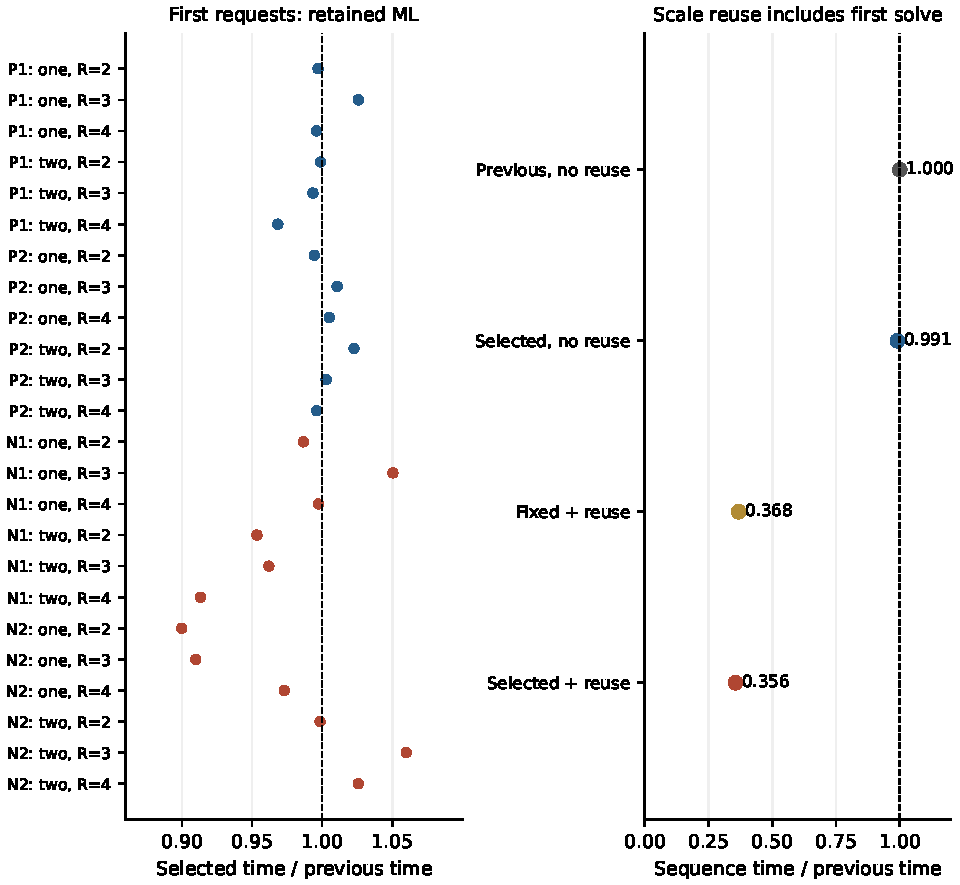
\includegraphics[width=\linewidth]{paper_figures/joint_policy_times.pdf}
\caption{Left: the selected-to-previous complete-time ratio for each reserved request, including slower cases. P and N identify the planar and nonplanar graphs, 1 and 2 identify the two kinematic profiles, and the labels give the numerator pattern and rank. Right: aggregate time for the four scale sequences, normalized to the preceding application without reuse. Every sequence includes its first Kira reduction. Dashed lines mark equal time. The panels have separate workloads and their ratios cannot be multiplied.}
\label{fig:joint-times}
\end{figure}
\FloatBarrier

\subsection{Exact reuse when only the overall scale changes}
For a massless family with homogeneous quadratic inverse propagators, a common positive change of all external scalar products gives an exact relation between reduction coefficients. If $\boldsymbol b_m$ is the index vector of master $m$, define $\nu(\boldsymbol a)=\sum_i a_i$. Then
\begin{equation}
 r_{\boldsymbol a m}(\lambda\boldsymbol x,d)
 =\lambda^{\nu(\boldsymbol b_m)-\nu(\boldsymbol a)}
  r_{\boldsymbol a m}(\boldsymbol x,d),\qquad\lambda>0.
 \label{eq:joint-scale-rule}
\end{equation}
Appendix~\ref{app:joint-policy} derives this identity by scaling the integration momenta. Its exponent is an integer, and a rational scale therefore gives an exact rational multiplier. The application checks the graph, target indices, supplied basis, and every dimensionless kinematic ratio before reusing an earlier result. Changed ratios, masses, or symbolic kinematic values continue through the reduction application. Reuse supplies no benefit before a matching exact result exists.

We test four predefined rank-four requests, two from each graph, in sequences with scale factors $1$, $3/2$, and $2$. Each sequence starts a fresh process and includes the initial Kira reduction, imports, model loading, input and output, exact transformation, and the subsequent independent coefficient checks. Three repetitions and four methods give 48 measured sequences containing 144 requests. Independent native reductions at every scale supply the checks; their coefficients never enter the application inputs.

We sum the median sequence times over the four base requests. Under this measure, the selected policy with scale reuse uses 28.496 seconds, compared with 80.073 seconds for the preceding application without reuse and 79.334 seconds for the selected policy without reuse. The resulting change relative to the preceding application is 64.4\% less time, with time-ratio interval $[0.334,0.390]$, while reuse alone changes the selected policy's time by 64.1\% less time, with time-ratio interval $[0.350,0.383]$. A fixed configuration with the same exact reuse uses 29.466 seconds; the selected-to-fixed-reuse comparison gives 3.3\% less time, with time-ratio interval $[0.770,1.049]$. All transformed outputs pass exact checks. These sequence results measure the benefit of repeated dimensionless kinematics, and remain separate from the first-request model comparison.

The deployed application combines the retained ML application with this exact reuse and retains the existing analytic and native paths outside its fitted domain. Eight further fresh-process checks reproduce the earlier four-loop native and eight-loop analytic results. These checks preserve existing behavior and do not extend the new model's fitted range. The new timing evidence covers known two-loop boxes, rational kinematics, symbolic dimension, and supplied bases. It does not establish a fastest possible strategy for arbitrary integrals or unrestricted loop order.
